\chapter{Aktueller Entwicklungsstand}

Dieses Kapitel soll einen Überblick über die aktuellen Entwicklungen im Bereich der Technologien, die für autonomes Fahren, speziell für die Positionsbestimmung, benötigt werden, vermitteln. Außerdem werden einige Projekte behandelt, die es sich zur auf Aufgabe gemacht haben, autonomes Fahren auf die weltweiten Straßen zu bringen.


\section{\acs{Lidar}-Entwicklung}

Die Entwicklung von Lidar-Scannern ist schreitet schneller voran als je zuvor. Eines der zahlreichen Unternehmen, die sich an der Entwicklung beteiligen, ist Ouster, ein US-amerikanisches Unternehmen, dessen Ziel es ist, ein massentaugliches Lidar-System zu einem relativ erschwinglichen Preis auf den Markt zu bringen. Derzeit bietet Ouster seinen \acs{Lidar}-Scanner \emph{OS-1} in drei verschiedenen Varianten mit 16, 64 oder 128 Kanälen an. Eine höhere Anzahl an Kanälen resultiert in einer höheren Auflösung, das Modell mit 16 Kanälen bietet eine Abtastrate von \num{327680} Punkten pro Sekunde, bei 128 Kanälen sind Abtastraten von \num{2621440} Punkten pro Sekunde möglich. Die Preise liegen zwischen \num{3500} und \num{18000} US-Dollar, für Non-Profit-Unternehmen und wissenschaftliche Einrichtungen gibt es zudem Vergünstigungen von bis zu 45 Prozent. \Vgl{ouster-web}

Aktueller Marktführer im Bereich der \acs{Lidar}-Scanner für autonome Fahrzeuge ist Velodyne LiDAR, dessen Produkte sich derzeit auf nahezu allen autonomen Testfahrzeugen befinden. Auch auf Vermessungsfahrzeugen für Kartendienstanbieter wie Google Maps, Apple Maps, TomTom oder Nokia Here, kommen die Syteme von Velodyne zum Einsatz. Der große Nachteil liegt allerdings beim Preis, der aufgrund des drehenden Lasers und damit verbunden den schwieriger herstellbaren beweglichen Teilen bei \num{75000} US-Dollar liegt. Der Trend steuert hier eindeutig in Richtung solid-state Lidar ohne bewegliche Teile, wodurch sich die Geräte deutlich einfacher und vor allem massentauglicher herstellen lassen. Allerdings muss erst eine Lösung dafür gefunden werden, den Laser in verschiedene Richtungen gleichzeitig bewegen zu lassen. Eine Möglichkeit ist ein sogenanntes \emph{phased array}, bei dem eine Reihe an Laser-Strahlen emittiert werden. Je nach Phase, also Gangunterschied, zwischen den einzelnen Emittern richtet sich der Laserstrahl in die entsprechende Richtung. Senden alle Emitter synchron, verläuft der resultierende Strahl geradeaus, sind jedoch die Emitter auf der linken Seite etwas nach hinten phasenverschoben, so verläuft auch der Laserstrahl etwas nach links gerichtet.
\Vgl{lidar-entwicklung}


\section{Nvidia DRIVE Localization}

Auf der jährlich in Las Vegas stattfindenden Consumer Electronics Show (CES) hat Nvidia, ein Unternehmen, welches eigentlich für High-End Grafikkarten bekannt ist, im Jänner 2019 eine offene Plattform namens \emph{Nvidia DRIVE Localization} vorgestellt. Das System basiert auf Nvidias hauseigenem, speziell für autonomes Fahren etwickelten Prozessor \emph{Nvidia DRIVE Xavier}, bei dem es sich um einen sogenannten \ac{SoC} handelt, welcher einen Deep Learning Accelerator und eine CUDA-Engine\footnote{\zit{cuda}{CUDA ist eine NVIDIA Architektur für parallele Berechnungen, die die Rechenleistung des Systems durch Nutzung der Leistung des Grafikprozessors deutlich steigern kann.}} beinhaltet. \Vgl{nvidia-drive}

Das System kommt dabei ohne jegliche \acs{Lidar}- oder \acs{Radar}-Scanner aus, es greift lediglich auf ein \ac{GNSS}, eine \ac{IMU} und den Tachometer des Fahrzeugs zurück. Neurale Netzte analysieren die Daten in Echtzeit und können verschiedenste Straßenmerkmale selbst in schlechten Wetterbedingungen auslesen. Diese Anforderungen können nur durch ernorme parallele Recheleistung, welche vom Xavier \ac{SoC} zur Verfügung gestellt wird, bewältigt werden. \Vgl{nvidia-drive}


\section{Waymo}

Waymo ist ein Schwesterunternehmen von Google und führt das im Jahr 2009 gegründete Projekt \emph{Google Driverless Car} fort. 2015 fand die erste, voll autonome Fahrt auf öffentlichen Straßen in Austin statt. Im Oktober 2018 erreichte Waymo den Meilenstein von 10 Millionen zurückgelegten Meilen (ca. 16 Millionen Kilometer) in ihrer Flotte von autonomen Fahrzeugen.

Am 5.\ Dezember 2018 startete Waymo ein kommerzielles Taxi-Service namens \emph{Waymo One} in vier Vororten von Phoenix, Arizona. Die autonomen Fahrzeuge werden derzeit noch von einem \enq{Sicherheitsfahrer} begleitet, der im Fall einer Fehlfunktion der autonomen Systeme, die Kontrolle über das Fahrzeug übernehmen kann \vgl{waymo-taxiservice}{}. Bereits seit 2017 bis zum Start von \emph{Waymo One} lief das sogenannte \emph{Early rider program}, an dem ausgewählte Bewohner des Ballungsraums von Phoenix teilnehmen konnten, um kostenlose Taxifahrten zu erhalten. Das Feedback der Teilnehmer trug zur Weiterentwicklung der autonomen Fahrzeuge bei.
\Vgl{waymo-website}


\section{Uber}

Auch der Fahrtendienst Uber hat im Februar 2015 bekanntgegeben, eine Flotte an autonomen Fahrzeugen aufzubauen um diese für Testfahrten zu benützten. Die ersten Tests starteten in Pittsburgh, sie wurden jedoch nach einiger Zeit aufgrund von Differenzen mit dem Bürgemeister der Stadt in Ubers Heimatstadt San Francisco verlegt. Seit 2017 finden auch, ebenso wie bei Waymo, Testfahrten im benachbarten Arizona statt. \Vgl{uber-tech-radar}

Bei einem Unfall im März 2017 in Tempe, Arizona wurde eine Frau von einem selbstfahrenden Uber-Fahrzeug, einem Volvo XC90, erfasst und dabei tödlich verletzt. Die Frau schob ihr Fahrrad über die vierspurige Straße, trotz Dunkelheit wurde sie aber von den zahlreichen Sensoren des Fahrzeug bereits sechs Sekunden vor dem Unfall erkannt. Das System war aber verwirrt, zuerst erkannte es die Frau als unbekanntes Objekt, dann als Fahrzeug und zuletzt als Fahrrad, dessen Pfad es nicht vorhersagen konnte. Nur 1,3 Sekunden vor dem Zusammenstoß erkannte das System, dass eine Notbremsung nötig war, führte diese jedoch nicht durch, da das automatische Notbremssystem deaktiviert war. Der Sicherheitsfahrer, der gerade auf einen Bildschirm des autonomen Systems schaute, konnte nicht mehr rechtzeitig Bremsen, wodurch das Fahrzeug ungebremst mit ungefähr \SI[per-mode=symbol]{60}{\kilo\metre\per\hour} auf das Opfer zufuhr. Nach dem Unfall wurden alle autonomen Testfahrten von Uber vorläufig eingestellt, nach rund einem Jahr wurden die Tests wieder fortgeführt.
\Vgl{uber-unfall}

Laut Uber CEO John Micklethwait sollen bereits ab Mitte 2019 erste Fahrten des Taxidienstes mit autonomen Fahrzeugen stattfinden. Zuerst allerdings nur in geringen Zahlen, in Phoenix beispielsweise sollen etwa fünf Prozent der Fahrten autonom sein, für die restlichen 95 Prozent reicht entweder das Material der annotierten digitalen Karten noch nicht aus oder die Wetterbedingungen sind für die Systeme noch zu anspruchsvoll. Nach und nach soll die Quote auf 100 Prozent angehoben werden, die Benutzer sollen dann auch auswählen können, ob sie lieber eine Fahrt mit einem autonomen Fahrzeug oder einem menschlichen Fahrer möchten.
\Vgl{uber-taxi}

\section{Tesla}

Tesla ist, ebenso wie Waymo, ein im Silicon Valley ansässiges Unternehmen mit folgendem selbst ernannten Ziel: \zit{tesla-about}{Die Beschleunigung des Übergangs zu nachhaltiger Energie.} Um dieses Ziel erreichen zu können, stellte Tesla im Jahr 2008 den Roadster vor, einen zweisitzigen Sportwagen, der die Finanzierung der Premium-Limousine Model S sicherte. Besondere Merkmale sind die größte Reichweite unter Elektrofahrzeugen und eine Beschleunigung von 0 auf 100 \si[per-mode=symbol]{\kilo\metre\per\hour} in 2,7 Sekunden. Derzeit läuft die Auslieferung der im Vergeleich zum Model S kompakteren Limousine Model 3, welches durch einen Grundpreis von \num{35000} US-Dollar die Verbreitung von Elektrofahrzeugen weiter vorantreiben soll.
\Vgl{tesla-about}

Teslas Fahrzeuge zählen außerdem zu den sichersten der Welt. Wie in \ref{safety-chart} zu sehen, sind von allen seit 2011 von der \ac{NHTSA} getesteten Fahrzeuge, die drei mit der niedrigsten Wahrscheinlichkeit von Verletzungen, alle von Tesla hergestellt. Das Model 3 hat hierbei einen besonders niedrigen Wert von nur 5,7 Prozent. Dieser Wert errechnet sich durch den \enq{Vehicle Safety Score} von 0,38 der mit der von der \ac{NHTSA} angegebenen Basiswahrscheinlichkeit von 15 Prozent multipliziert wird. \Vgls[40038]{nhtsa-baseline}{model-3-score}

\begin{figure}\centering
  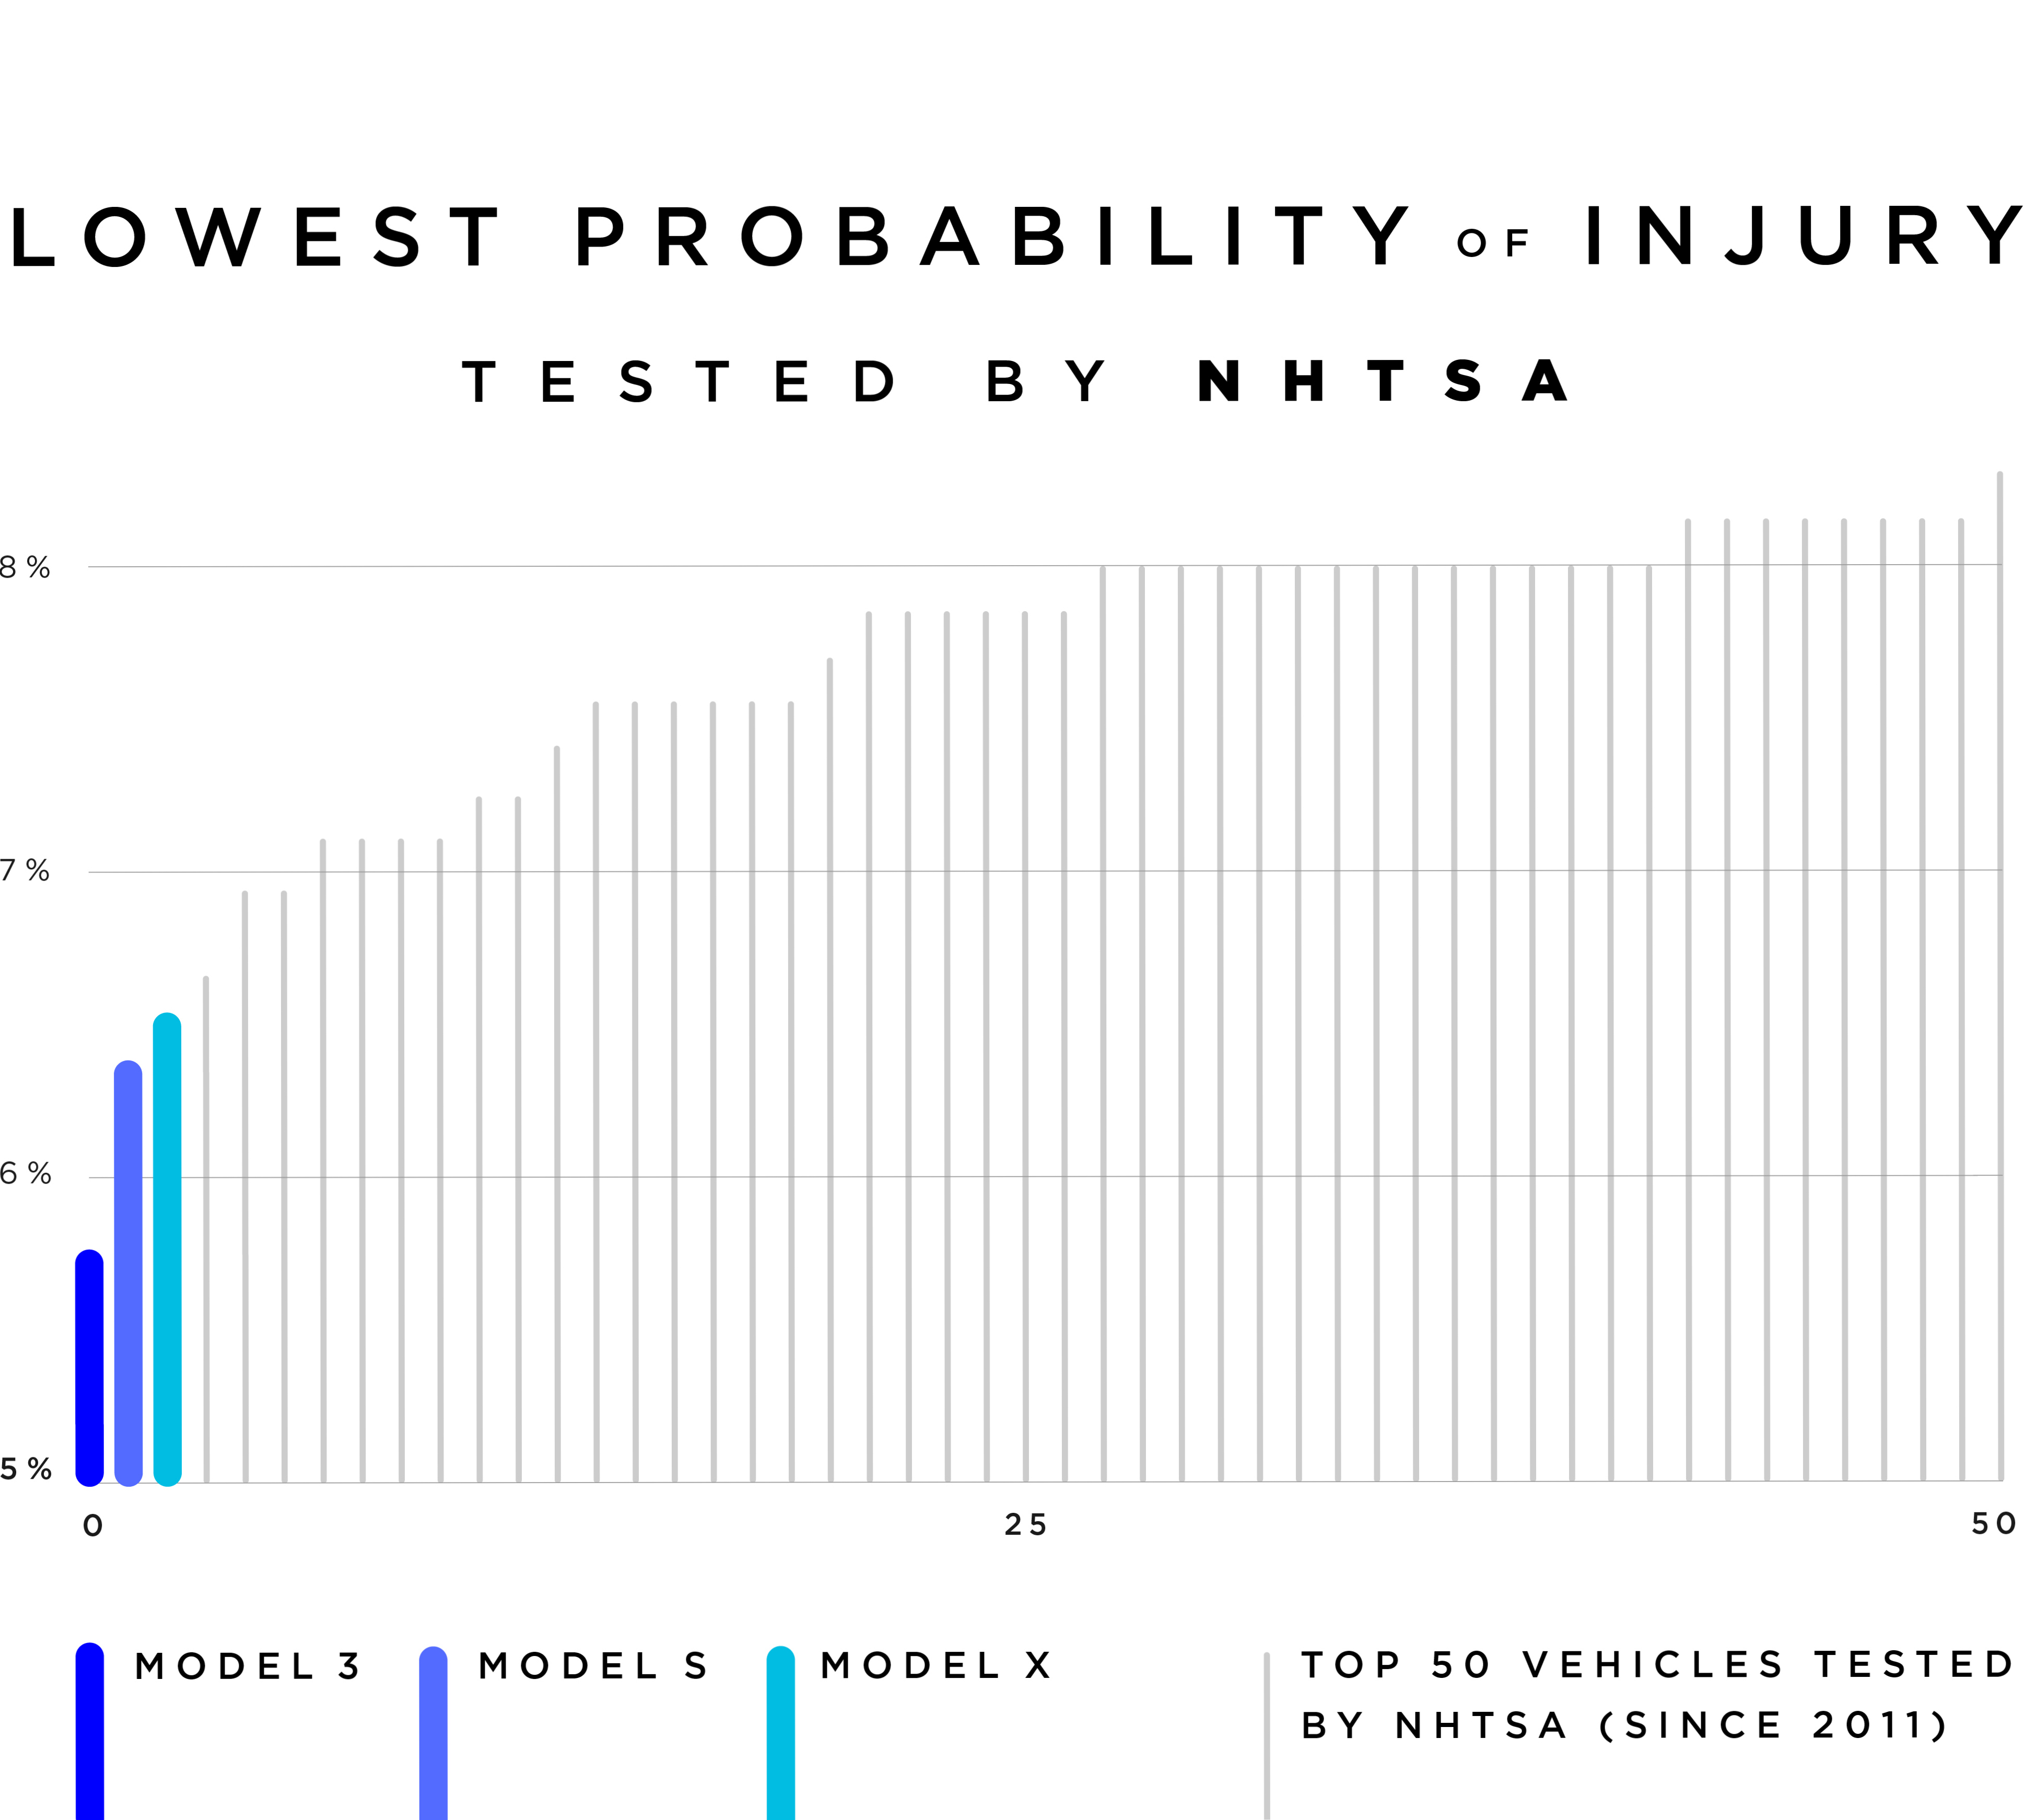
\includegraphics[width=\textwidth]{safety-chart.jpg}
  \captionbelow[Niedrigste Wahrscheinlichkeit von Verletzungen. Getestet von der \ac{NHTSA}. Bildquelle: \fullcite{tesla-safety}]{Niedrigste Wahrscheinlichkeit von Verletzungen. Getestet von der \ac{NHTSA} (\cite{tesla-safety})}
  \label{safety-chart}
\end{figure}

Weiters ist Tesla für seinen bereits in \ref{section-2-3} behandelten Autopilot. Am 27.\ November haben Teslas Fahrzeuge eine Milliarde Meilen (ca. 1,6 Milliarden Kilometer) mit aktiviertem Autopilot zurückgelegt. Das entspricht etwa 10 Prozent aller von Teslas Fahrzeuges weltweit gefahrenen Meilen, wobei hierbei auch Fahrzeuge ohne Autopilot-Hardware bzw. solche mit Hardware, jedoch ohne der notwendigen kostenpflichtigen Aktivierung des Assistenzsystems miteingerechnet werden. \Vgl{electrek-one-billion}


\section{Wiener Linien}

Im Frühjahr 2019 soll die erste autonome Buslinie Wiens in der Seestadt in Betrieb gehen. Das Projekt namens \emph{auto.Bus - Seestadt} durchläuft derzeit intensive Testfahrten auf geschlossenem Gelände. Bei dem Bus handelt es sich um einen vollelektrischen Kleinbus (siehe \ref{bus-seestadt}), der Platz für bis zu zehn Fahrgäste und einen Operator bietet. Der Operator ist derzeit noch aus sicherheitsgründen notwendig, er überwacht den Bus und kann im Ernstfall ins Geschehen eingreifen. \Vgl{wiener-linien}

\begin{figure}\centering
  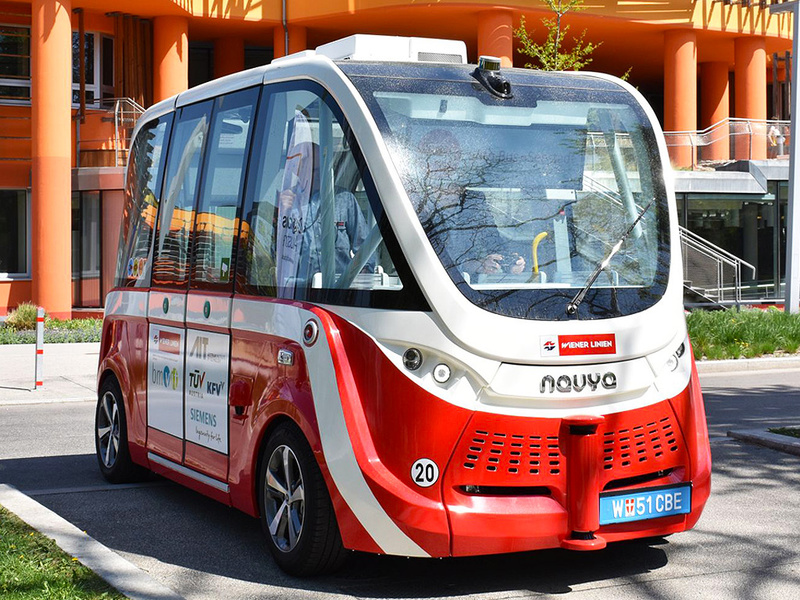
\includegraphics[width=\textwidth-1cm]{bus-seestadt.jpg}
  \captionbelow[Elektrischer Kleinbus der Wiener Linien. Bildquelle: \fullcite{wiener-linien}]{Elektrischer Kleinbus der Wiener Linien (\cite{wiener-linien})}
  \label{bus-seestadt}

  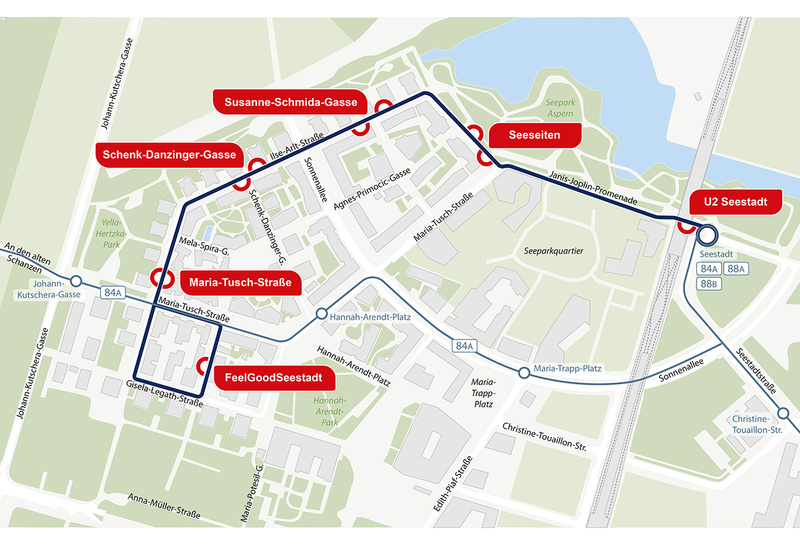
\includegraphics[width=\textwidth-1cm]{bus-seestadt-karte.jpg}
  \captionbelow[Geplante Route der autonomen Buslinie. Bildquelle: \fullcite{wiener-linien}]{Geplante Route der autonomen Buslinie (\cite{wiener-linien})}
  \label{bus-seestadt-karte}
\end{figure}

Die geplante Route ist in \ref{bus-seestadt-karte} dargestellt, sie ist 2 \si{\kilo\metre} lang und bedient sechs Stationen in der Seestadt. Die Beförderung auf der Linie ist kostenlos. Da es sich um einen Testbetrieb handelt, ist der Transport von Kinderwägen und Rollstühlen rechtlich nicht erlaubt.
\Vgl{wiener-linien}


\section{Aktionspaket des Bundesministeriums für Verkehr, Innovation und Technologie}

Das \ac{bmvit} veröffentliche im November 2018 sein \emph{Aktionspaket Automatisierte Mobilität. 2019 -- 2022}, in dem Österreichs Ziele und Maßnahmen zur Verbreitung von autonomem Fahren dargelegt werden.

Durch eine Novelle des Kraftfahrgesetztes im Jahr 2016, wurden die rechtlichen Rahmenbedingungen geschaffen, um \enq{ALP.Lab} (Austrian Light Vehicle Proving Region for Automated Driving), Österreichs erste Testumgebung für autonome Fahrzeuge, in der Steiermark zu errichten. Durch Erstellung der Verordnung zum automatisierten Fahren konnten außerdem erstmals Test auf öffentlichen Straßen durchgeführt werden \vgl{automat-fahr-v}{}. Hierbei werden insbesondere Autobahnpiloten mit automatischem Spurwechsel, selbstfahrende Heeresfahrzeuge und autonome Kleinbusse getestet.
\Vgl[10]{bmvit}

Das \ac{bmvit} strebt einen \zit[23]{bmvit}{verkehlich sinnvollen und effizienten Einsatz automatisierter Mobilität sowie die Stärkung der Wettbewerbsposition Österreichs} an. In erster Linie gehe es allerdings laut Aktionsplan um \zit[23]{bmvit}{lebenswerte öffentliche Räume.} Diese Punkte will die Regierung besonders durch Testen und Pilotieren erreichen, wobei der Nutzer Mittelpunkt dieser Tests sein soll. Letztendlich muss nämlich der Verkehr für alle die an ihm teilnehmen eines werden: sicherer. Insbesondere schwächere Verkehrsteilnehmer wie Radfahrer oder Fußgänger sollen in ihrer Sicherheit gestärkt werden.

Ein weiteres wichtiges Anliegen ist die Reduktion der \ce{CO2}-Emissionen im Verkehrssektor, bis 2050 soll Österreichs Verkehr vollständig \ce{CO2}-neutral werden. Das ist nicht nur durch den Einsatz elektrischer Fahrzeuge erreichbar, sondern auch durch autonome Mobilität. Die Notwendigkeit eines eigenen Fahrzeuges ist durch autonome Taxis, die rund um die Uhr von jedermann verwendet werden können, nicht mehr so hoch wie heute.
\Vgl[24]{bmvit}
